\documentclass[11pt,a4paper]{article}
\usepackage[utf8]{inputenc}
\usepackage[T1]{fontenc}
\usepackage{geometry}
\usepackage{titlesec}
\usepackage{enumitem}
\usepackage{xcolor}
\usepackage{fancyhdr}
\usepackage{fontawesome}
\usepackage{hyperref}
\usepackage{graphicx}
\usepackage{tcolorbox}
\usepackage{multicol}
\usepackage{setspace}

% Page setup
\geometry{
    left=1.5cm,
    right=1.5cm,
    top=1.5cm,
    bottom=1.5cm
}

% Colors
\definecolor{primarygreen}{HTML}{36b41f}
\definecolor{darkgreen}{HTML}{2d4d2d}
\definecolor{lightgreen}{HTML}{8a9a8a}
\definecolor{textdark}{HTML}{000000}
\definecolor{textlight}{HTML}{666666}
\definecolor{bglight}{HTML}{f8f9fa}

% Hyperlink setup
\hypersetup{
    colorlinks=true,
    urlcolor=primarygreen,
    linkcolor=primarygreen
}

% Header formatting
\titleformat{\section}
    {\Large\bfseries\color{primarygreen}}
    {}{0em}{}[\titlerule]

\titleformat{\subsection}
    {\large\bfseries\color{textdark}}
    {}{0em}{}

% Custom commands
\newcommand{\contactitem}[2]{\textbf{#1} #2}
\newcommand{\skilltag}[1]{\textcolor{white}{\textbf{#1}}}

% Header
\fancypagestyle{plain}{
    \fancyhf{}
    \renewcommand{\headrulewidth}{0pt}
}

% Document begin
\begin{document}
\pagestyle{plain}

% Header section with gradient effect
\begin{tcolorbox}[
    colback=primarygreen,
    coltext=white,
    boxrule=0pt,
    arc=0pt,
    left=0pt,
    right=0pt,
    top=0pt,
    bottom=0pt,
    width=\textwidth
]
\begin{center}
\vspace{0.5cm}

% Profile section
\begin{minipage}{0.25\textwidth}
\centering
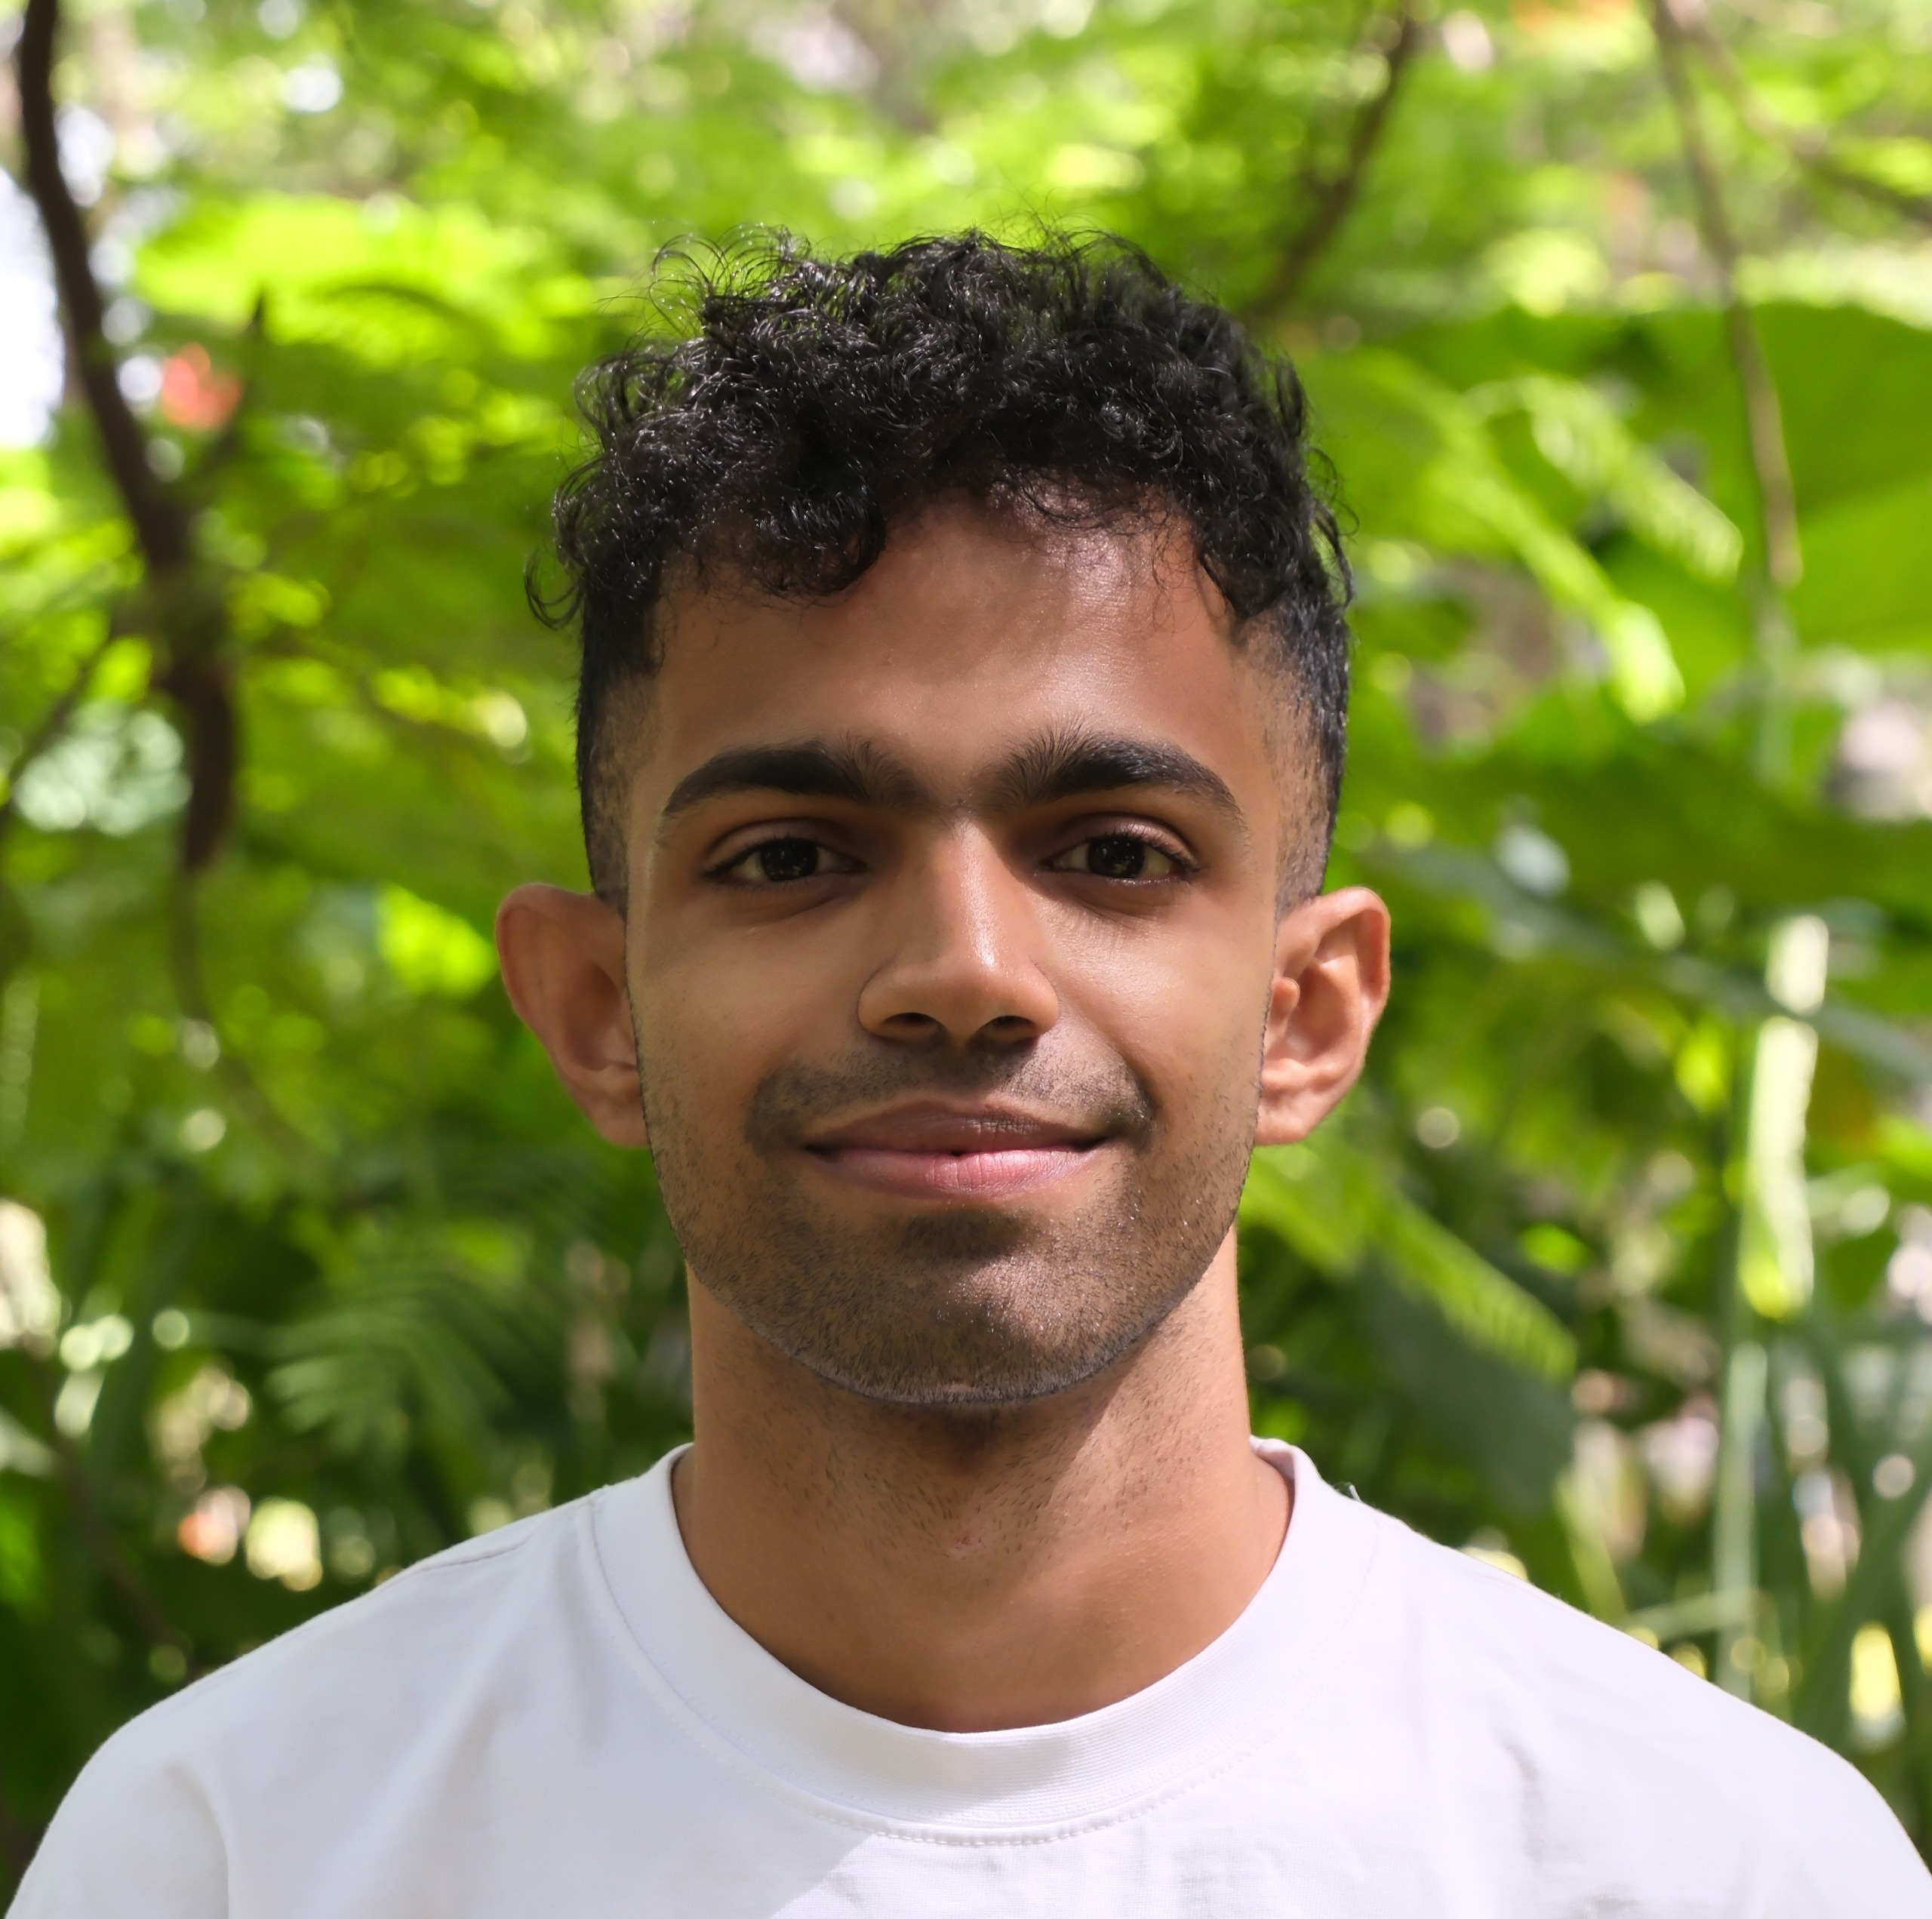
\includegraphics[width=3cm,height=3cm,keepaspectratio]{headshot.jpg}
\end{minipage}
\begin{minipage}{0.7\textwidth}
\raggedright

{\Huge\textbf{ARJUN SHENOY}}\\[0.3cm]
{\Large Full Stack Developer}\\[0.5cm]

% Contact information
\begin{multicols}{2}
\begin{itemize}[leftmargin=*]
    \item \faPhone\ (+91) 79945-61953
    \item \faEnvelope\ tech.noishey@gmail.com
    \item \faLinkedin\ \href{https://linkedin.com/in/noishey}{linkedin.com/in/noishey}
    \item \faMapMarker\ Bengaluru, India
    \item \faGlobe\ \href{https://www.noishey.tech}{www.noishey.tech}
\end{itemize}
\end{multicols}

\end{minipage}
\end{center}
\vspace{0.5cm}
\end{tcolorbox}

\vspace{0.5cm}

% Summary section
\section{SUMMARY}
I am Arjun, also known as Noishey, my online character. I'm interested in technology, particularly developing web2/web3 tools and applications. I also have a keen sense of design and am interested in topics like finance, blockchain, and retrieval augmented generation (RAG). I want to work for a startup that is expanding sustainably and uses modern technology so that I can get my hands working and use my abilities to help the company develop. I provide all of the useful tech abilities I've acquired from my time in college to my most current full-time tech freelancing work.

% Skills section
\section{SKILLS}
\begin{center}
\begin{tcolorbox}[
    colback=bglight,
    colframe=primarygreen,
    boxrule=0.5pt,
    arc=0pt,
    width=\textwidth
]
\begin{multicols}{4}
\begin{itemize}[leftmargin=*]
    \item \skilltag{JavaScript}
    \item \skilltag{React.js}
    \item \skilltag{TypeScript}
    \item \skilltag{Node.js}
    \item \skilltag{TailwindCSS}
    \item \skilltag{Supabase}
    \item \skilltag{Express.js}
    \item \skilltag{UI/UX}
    \item \skilltag{LLM Prompting}
    \item \skilltag{MongoDB}
    \item \skilltag{Next.js}
    \item \skilltag{GraphQL}
    \item \skilltag{Vercel}
    \item \skilltag{Docker}
    \item \skilltag{Kubernetes}
    \item \skilltag{CI/CD}
    \item \skilltag{Ether.js}
    \item \skilltag{Metamask}
    \item \skilltag{NexAuth.js}
    \item \skilltag{AWS}
\end{itemize}
\end{multicols}
\end{tcolorbox}
\end{center}

% Projects section
\section{PROJECTS}

\subsection{Rortal}
\textit{AI Generated Gradients to NFT's}\\[0.2cm]
It is a web application written using Javascript and built on Next.js platform. I used Stable Diffusion API to retrieve gradients through pre-defined set of parameters like glow, fluidity and noise. I enabled wallet integration using Metamask.

\subsection{Shadow}
\textit{AI Assistant for Mental Health Therapy}\\[0.2cm]
What was a successful outcome of your work? (e.g. Raised \$3,000 for the charity)

\subsection{Ground}
\textit{Regression Model to predict soil quality}\\[0.2cm]
What was a successful outcome of your work? (e.g. Raised \$3,000 for the charity)

% Experience section
\section{EXPERIENCE}

\subsection{Software Engineer}
\textit{Invesco}\hfill \faCalendar\ 07/2022 - 11/2023\\
\faMapMarker\ Hyderabad, India\\[0.2cm]
Completed a year-long rotational training program across multiple teams in major tech hubs where the company operates. Gained broad exposure to various technologies and collaborated with global team members. Contributed to projects involving JavaScript technologies such as React and Next.js.

\subsection{Freelancer}
\textit{Self Employed}\hfill \faCalendar\ 2023 - Present\\
\faMapMarker\ Remote\\[0.2cm]
Prioritized JavaScript-first development after transitioning from a full-time role, focusing on building and learning with modern web technologies. Secured multiple clients globally for both minor and major projects through organic reach and professional networking.

% Education section
\section{EDUCATION}

\subsection{Bachelor's, Computer Science Engineering}
\textit{Model Engineering College, Kochi}\hfill \faCalendar\ 2018 - 2022

\end{document}
